\documentclass{standalone}
\usepackage{tikz}
\usetikzlibrary{patterns, positioning}
\usepackage[sfdefault]{ClearSans} %% option 'sfdefault' activates Clear Sans as the default text font
\usepackage[T1]{fontenc}

\begin{document}
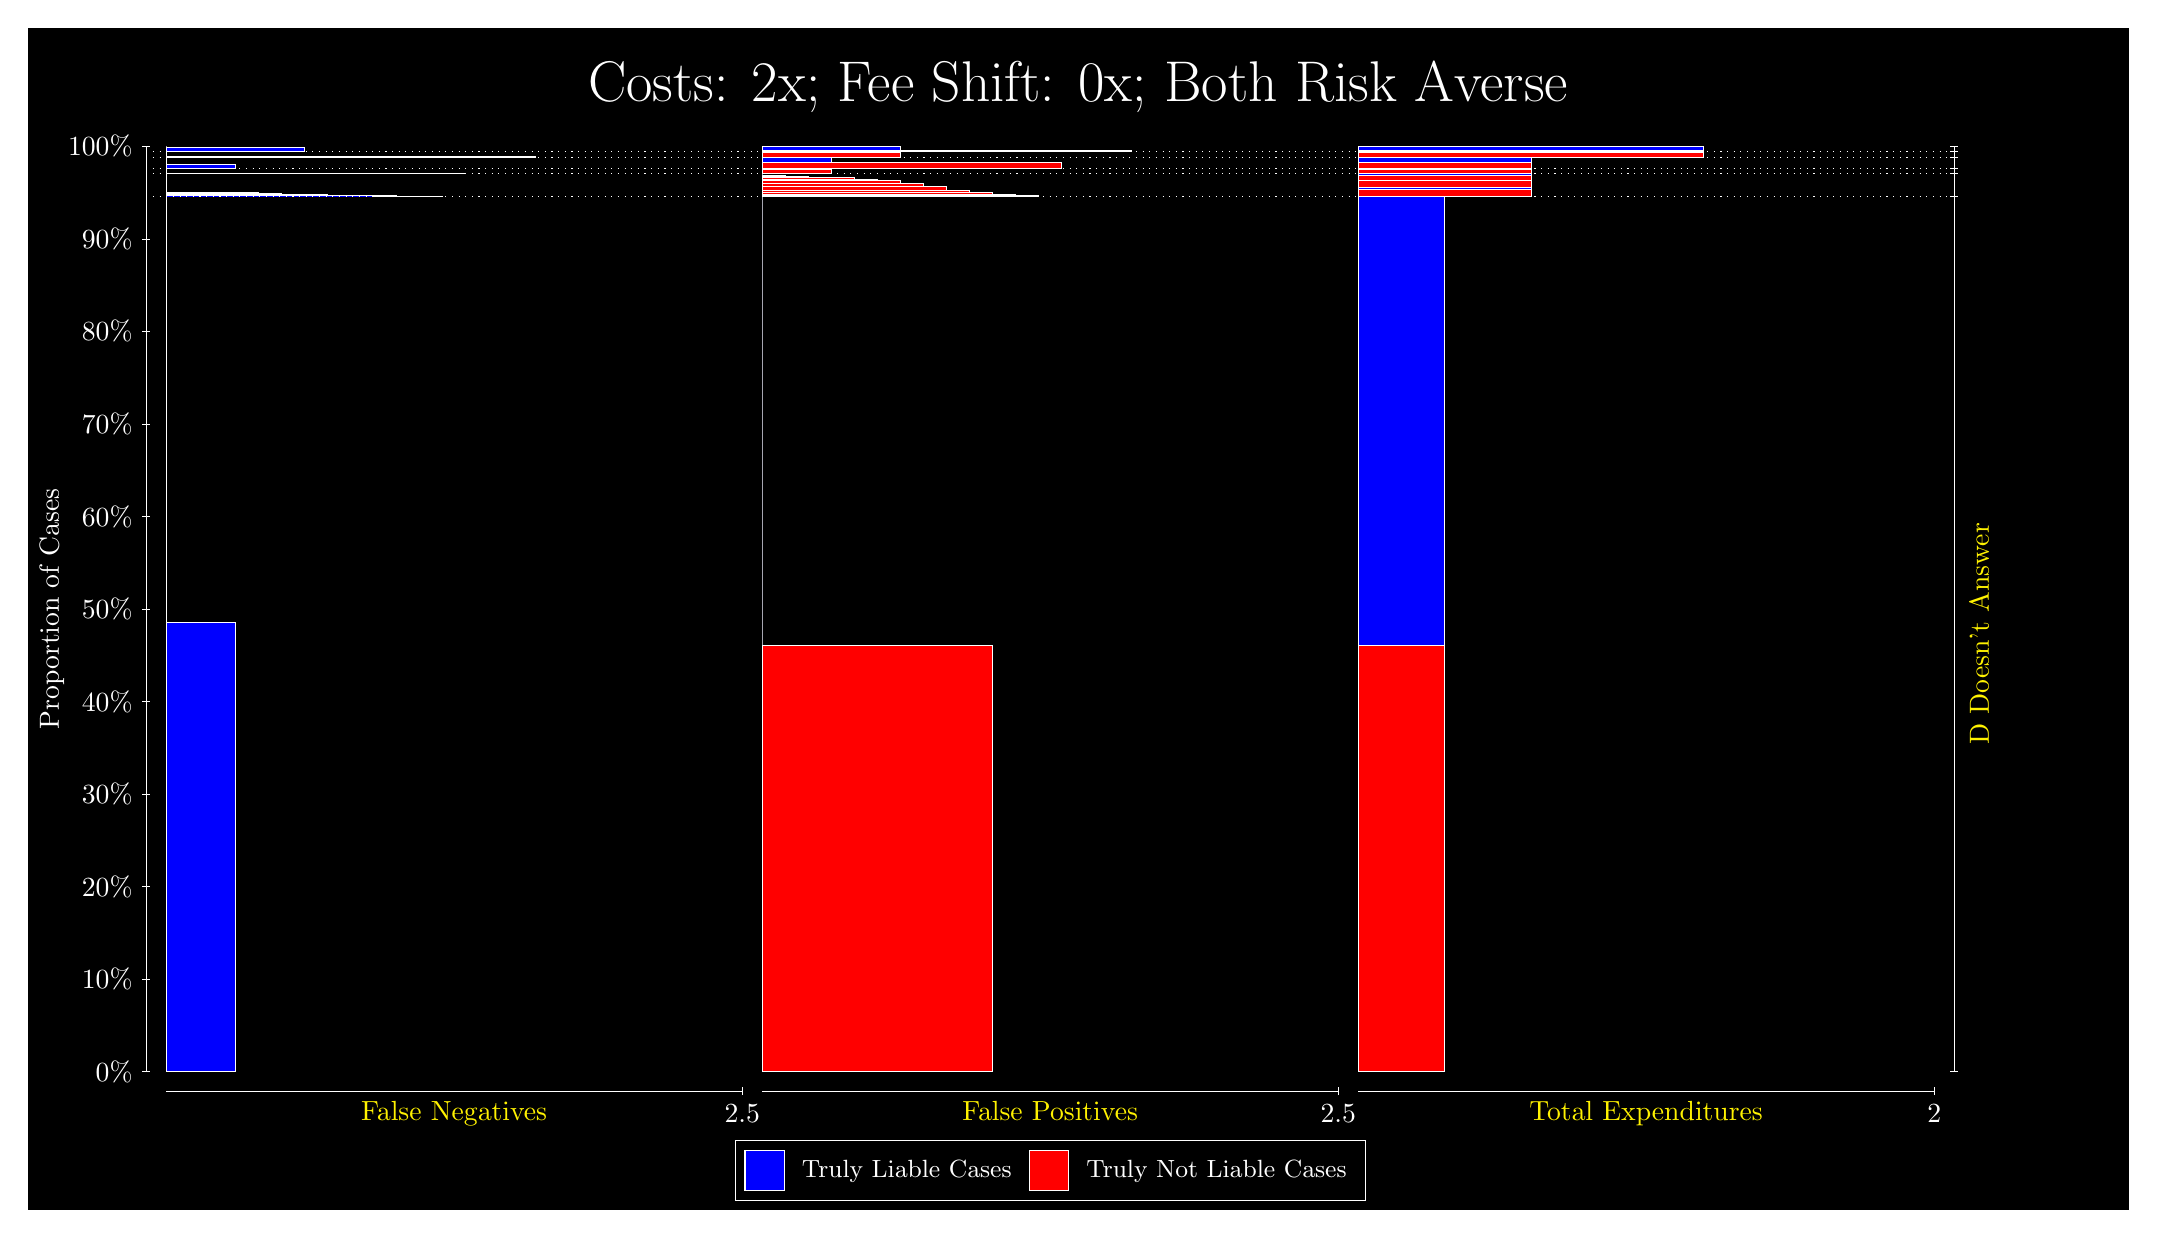
\begin{tikzpicture}
\draw[fill=black] (0,0) rectangle (26.667,15);
\draw[text=white] (0,13.5) rectangle (26.667,15) node[midway] {\huge Costs: 2x; Fee Shift: 0x; Both Risk Averse};
\draw[white, very thin] (1.5,1.75) -- (1.5,13.5);
\node[rotate=90, text=white, anchor=center] at (0.3, 7.625) {Proportion of Cases};
\draw[white, very thin] (1.45,1.75) -- (1.55,1.75);
\node[text=white, anchor=east] at (1.45, 1.75) {0\%};
\draw[white, very thin] (1.45,2.925) -- (1.55,2.925);
\node[text=white, anchor=east] at (1.45, 2.925) {10\%};
\draw[white, very thin] (1.45,4.1) -- (1.55,4.1);
\node[text=white, anchor=east] at (1.45, 4.1) {20\%};
\draw[white, very thin] (1.45,5.275) -- (1.55,5.275);
\node[text=white, anchor=east] at (1.45, 5.275) {30\%};
\draw[white, very thin] (1.45,6.45) -- (1.55,6.45);
\node[text=white, anchor=east] at (1.45, 6.45) {40\%};
\draw[white, very thin] (1.45,7.625) -- (1.55,7.625);
\node[text=white, anchor=east] at (1.45, 7.625) {50\%};
\draw[white, very thin] (1.45,8.8) -- (1.55,8.8);
\node[text=white, anchor=east] at (1.45, 8.8) {60\%};
\draw[white, very thin] (1.45,9.975) -- (1.55,9.975);
\node[text=white, anchor=east] at (1.45, 9.975) {70\%};
\draw[white, very thin] (1.45,11.15) -- (1.55,11.15);
\node[text=white, anchor=east] at (1.45, 11.15) {80\%};
\draw[white, very thin] (1.45,12.325) -- (1.55,12.325);
\node[text=white, anchor=east] at (1.45, 12.325) {90\%};
\draw[white, very thin] (1.45,13.5) -- (1.55,13.5);
\node[text=white, anchor=east] at (1.45, 13.5) {100\%};

\draw[white, very thin] (24.457,1.75) -- (24.457,13.5);
\draw[white, very thin] (24.407,1.75) -- (24.507,1.75);
\node[anchor=west] at (24.407, 1.75) {};
\draw[white, very thin] (24.407,12.866) -- (24.507,12.866);
\node[anchor=west] at (24.407, 12.866) {};
\draw[white, very thin] (24.407,13.158) -- (24.507,13.158);
\node[anchor=west] at (24.407, 13.158) {};
\draw[white, very thin] (24.407,13.215) -- (24.507,13.215);
\node[anchor=west] at (24.407, 13.215) {};
\draw[white, very thin] (24.407,13.356) -- (24.507,13.356);
\node[anchor=west] at (24.407, 13.356) {};
\draw[white, very thin] (24.407,13.439) -- (24.507,13.439);
\node[anchor=west] at (24.407, 13.439) {};
\draw[white, very thin] (24.407,13.5) -- (24.507,13.5);
\node[anchor=west] at (24.407, 13.5) {};

\draw[white, very thin, fill=blue] (1.75,1.75) rectangle (2.6283,7.4509);
\draw[white, very thin, fill=red] (1.75,7.4509) rectangle (1.75,12.866);
\draw[white, very thin, fill=blue] (1.75,12.866) rectangle (5.2631,12.869);
\draw[white, very thin, fill=blue] (1.75,12.869) rectangle (4.9703,12.87);
\draw[white, very thin, fill=blue] (1.75,12.87) rectangle (4.6775,12.874);
\draw[white, very thin, fill=blue] (1.75,12.874) rectangle (4.3848,12.875);
\draw[white, very thin, fill=blue] (1.75,12.875) rectangle (4.3848,12.879);
\draw[white, very thin, fill=blue] (1.75,12.879) rectangle (4.092,12.884);
\draw[white, very thin, fill=blue] (1.75,12.884) rectangle (3.7993,12.888);
\draw[white, very thin, fill=blue] (1.75,12.888) rectangle (3.5065,12.895);
\draw[white, very thin, fill=blue] (1.75,12.895) rectangle (3.2138,12.9);
\draw[white, very thin, fill=blue] (1.75,12.9) rectangle (2.921,12.913);
\draw[white, very thin, fill=red] (1.75,12.913) rectangle (1.75,13.158);
\draw[white, very thin, fill=blue] (1.75,13.158) rectangle (5.5558,13.162);
\draw[white, very thin, fill=red] (1.75,13.162) rectangle (1.75,13.215);
\draw[white, very thin, fill=blue] (1.75,13.215) rectangle (2.6283,13.274);
\draw[white, very thin, fill=red] (1.75,13.274) rectangle (1.75,13.356);
\draw[white, very thin, fill=blue] (1.75,13.356) rectangle (6.4341,13.372);
\draw[white, very thin, fill=red] (1.75,13.372) rectangle (1.75,13.439);
\draw[white, very thin, fill=blue] (1.75,13.439) rectangle (3.5065,13.486);
\draw[white, very thin, fill=red] (1.75,13.486) rectangle (1.75,13.5);
\draw[white, very thin, fill=red] (9.3189,1.75) rectangle (12.246,7.1647);
\draw[white, very thin, fill=blue] (9.3189,7.1647) rectangle (9.3189,12.866);
\draw[white, very thin, fill=red] (9.3189,12.866) rectangle (12.832,12.872);
\draw[white, very thin, fill=red] (9.3189,12.872) rectangle (12.539,12.885);
\draw[white, very thin, fill=red] (9.3189,12.885) rectangle (12.246,12.912);
\draw[white, very thin, fill=red] (9.3189,12.912) rectangle (11.954,12.943);
\draw[white, very thin, fill=red] (9.3189,12.943) rectangle (11.661,12.994);
\draw[white, very thin, fill=red] (9.3189,12.994) rectangle (11.368,13.031);
\draw[white, very thin, fill=red] (9.3189,13.031) rectangle (11.075,13.067);
\draw[white, very thin, fill=red] (9.3189,13.067) rectangle (10.783,13.079);
\draw[white, very thin, fill=red] (9.3189,13.079) rectangle (10.49,13.111);
\draw[white, very thin, fill=blue] (9.3189,13.111) rectangle (9.9044,13.124);
\draw[white, very thin, fill=blue] (9.3189,13.124) rectangle (9.6116,13.129);
\draw[white, very thin, fill=blue] (9.3189,13.129) rectangle (9.3189,13.158);
\draw[white, very thin, fill=red] (9.3189,13.158) rectangle (10.197,13.21);
\draw[white, very thin, fill=blue] (9.3189,13.21) rectangle (9.3189,13.215);
\draw[white, very thin, fill=red] (9.3189,13.215) rectangle (13.125,13.296);
\draw[white, very thin, fill=blue] (9.3189,13.296) rectangle (10.197,13.356);
\draw[white, very thin, fill=red] (9.3189,13.356) rectangle (11.075,13.423);
\draw[white, very thin, fill=blue] (9.3189,13.423) rectangle (9.3189,13.439);
\draw[white, very thin, fill=red] (9.3189,13.439) rectangle (14.003,13.453);
\draw[white, very thin, fill=blue] (9.3189,13.453) rectangle (11.075,13.5);
\draw[white, very thin, fill=red] (16.888,1.75) rectangle (17.986,7.1647);
\draw[white, very thin, fill=blue] (16.888,7.1647) rectangle (17.986,12.866);
\draw[white, very thin, fill=red] (16.888,12.866) rectangle (19.083,12.957);
\draw[white, very thin, fill=blue] (16.888,12.957) rectangle (19.083,12.974);
\draw[white, very thin, fill=red] (16.888,12.974) rectangle (19.083,13.065);
\draw[white, very thin, fill=blue] (16.888,13.065) rectangle (19.083,13.074);
\draw[white, very thin, fill=red] (16.888,13.074) rectangle (19.083,13.138);
\draw[white, very thin, fill=blue] (16.888,13.138) rectangle (19.083,13.158);
\draw[white, very thin, fill=red] (16.888,13.158) rectangle (19.083,13.21);
\draw[white, very thin, fill=blue] (16.888,13.21) rectangle (19.083,13.215);
\draw[white, very thin, fill=red] (16.888,13.215) rectangle (19.083,13.296);
\draw[white, very thin, fill=blue] (16.888,13.296) rectangle (19.083,13.356);
\draw[white, very thin, fill=red] (16.888,13.356) rectangle (21.279,13.423);
\draw[white, very thin, fill=blue] (16.888,13.423) rectangle (21.279,13.439);
\draw[white, very thin, fill=red] (16.888,13.439) rectangle (21.279,13.453);
\draw[white, very thin, fill=blue] (16.888,13.453) rectangle (21.279,13.5);
\draw[white, dotted] (1.5,12.866) -- (24.457,12.866);
\draw[white, dotted] (1.5,13.158) -- (24.457,13.158);
\draw[white, dotted] (1.5,13.215) -- (24.457,13.215);
\draw[white, dotted] (1.5,13.356) -- (24.457,13.356);
\draw[white, dotted] (1.5,13.439) -- (24.457,13.439);
\draw[white, very thin] (1.75,1.5) -- (9.0689,1.5);
\node[text=yellow, anchor=north] at (5.4094, 1.5) {False Negatives};
\draw[white, very thin] (9.0689,1.45) -- (9.0689,1.55);
\node[text=white, anchor=north] at (9.0689, 1.45) {2.5};

\draw[white, very thin] (9.3189,1.5) -- (16.638,1.5);
\node[text=yellow, anchor=north] at (12.978, 1.5) {False Positives};
\draw[white, very thin] (16.638,1.45) -- (16.638,1.55);
\node[text=white, anchor=north] at (16.638, 1.45) {2.5};

\draw[white, very thin] (16.888,1.5) -- (24.207,1.5);
\node[text=yellow, anchor=north] at (20.547, 1.5) {Total Expenditures};
\draw[white, very thin] (24.207,1.45) -- (24.207,1.55);
\node[text=white, anchor=north] at (24.207, 1.45) {2};

\node[text=yellow, centered, rotate=90] at (24.777, 7.3078) {D Doesn't Answer};






\draw (12.978300999999998,1.5) node[draw=none] (baseCoordinate) {};
\begin{scope}[align=center]
        \matrix[scale=0.5, draw=white, below=0.5cm of baseCoordinate, nodes={draw}, column sep=0.1cm]{
            \node[rectangle, draw, minimum width=0.5cm, minimum height=0.5cm, fill=blue] {}; &
            \node[draw=none, font=\small, text=white] (B) {Truly Liable Cases}; &
            \node[rectangle, draw, minimum width=0.5cm, minimum height=0.5cm, fill=red] {}; &
            \node[draw=none, font=\small, text=white] (B) {Truly Not Liable Cases}; \\
            };
\end{scope}

\end{tikzpicture}
\end{document}